\setcounter{section}{-1}
\section{The Era Before}
Historians date the origin of computing far back almost in the middle age. Here we
prefer to start when computers became commercially available and started to play
a role in business and science. This was around 1960 or even slightly before. Only
a few inventions had caused this development.

\begin{description}
  \item On the \emph{physical} level, it had been the advent of electronics that
  made computers objects of interest. Electronics offered the necessary speed. Up
  to these times, the active elements of electronic circuits were vacuum tubes.
  Heated cathodes emitted electrons, sucked up by the surrounding anode. In
  between a grid allowed to control the flow of electrons by applying a negative
  field. Early computers contained thousands of such tubes which, due the cathode
  heating and the high voltage at the anode consumed a considerable amount of
  energy, a few Watts every tube. With their numerous tubes and heavy power
  supplies, these early computers were quite monstrous and filled entire rooms.

  \item On the \emph{logical} level, the innovation of John von Neumann (1944) made
  computers into what they are. Before, they typically consisted of a control unit
  and a separate arithmetic unit. The former fetched instructions from an instruction
  store one after the other, the latter interpreted them and accordingly altered data
  in the data store.
  \begin{figure}[h!]
    \flushright
    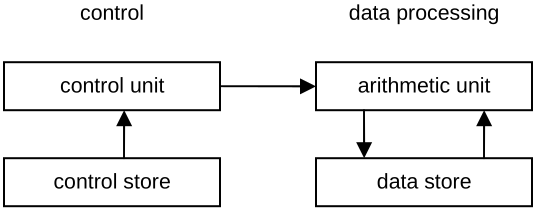
\includegraphics[width=.8\textwidth]{i/0}
  \end{figure}

  von Neumann introduced 2 fundamental concepts:
  \begin{enumerate}
    \item The 2 stores were united. This allowed the computer to generate data and
    then interpret them as instructions. Thereby, the computer mutated from a special
    purpose device (with always the same program) to a universal machine, the
    programmable computer. And this is what distinguishes the computer from all other
    technical devices up to this day.

    \item The conditional instruction. It has a different result depending on
    previously computed values, i.e. the state of the machine.
  \end{enumerate}
  Experimental computers developed as prototypes, usually at universities, between
  1945 and 1960, all adopted these 2 ideas.
\end{description}
